% Template based on:
% https://www.cs.columbia.edu/~djhsu/coms4774-s21/scribe.html

\documentclass[12pt]{article}

\usepackage{physics}
\usepackage{dsfont}
\usepackage{amscd}
\usepackage{amsmath}
\usepackage{amssymb}
\usepackage{amstext}
\usepackage{amsthm}
\usepackage{bbold}
\usepackage{bm}
\usepackage{colonequals}
\usepackage[dvips,letterpaper,margin=1in]{geometry}
\usepackage{mathtools}
\usepackage{graphicx}
\usepackage{xcolor}

\usepackage{csquotes}
\MakeOuterQuote{"}

\definecolor{cblack}{rgb}{0,0,0}
\definecolor{cblue}{rgb}{0.121569,0.466667,0.705882}
\definecolor{corange}{rgb}{1.000000,0.498039,0.054902}
\definecolor{cgreen}{rgb}{0.172549,0.627451,0.172549}
\definecolor{cred}{rgb}{0.839216,0.152941,0.156863}
\definecolor{cpurple}{rgb}{0.580392,0.403922,0.741176}
\definecolor{cbrown}{rgb}{0.549020,0.337255,0.294118}
\definecolor{cpink}{rgb}{0.890196,0.466667,0.760784}
\definecolor{cgray}{rgb}{0.498039,0.498039,0.498039}

\usepackage{hyperref}
\hypersetup{
  linkcolor  = cblue,
  citecolor  = cgreen,
  urlcolor   = corange,
  colorlinks = true,
}
\usepackage[capitalise,noabbrev,nameinlink]{cleveref}

% Lecture information
\newcommand\coursename{CPSC 664, Spring 2023}
\newcommand\scribe{Felix Zhou}
\newcommand\lecturer{Tim Kunisky}
\newcommand\lecturedate{February 14, 2023}
\newcommand\lecturetitle{LECTURE \#9: FIXME}

% Define theorem environments here.
\newtheorem{claim}{Claim}
\newtheorem{theorem}{Theorem}[section]
\newtheorem{remark}[theorem]{Remark}
\newtheorem{assumption}[theorem]{Assumption}
\newtheorem{lemma}[theorem]{Lemma}
\newtheorem{question}[theorem]{Question}
\newtheorem{problem}[theorem]{Problem}
\newtheorem{definition}[theorem]{Definition}
\newtheorem{example}[theorem]{Example}
\newtheorem{proposition}[theorem]{Proposition}
\newtheorem{corollary}[theorem]{Corollary}
\newtheorem{conjecture}[theorem]{Conjecture}

% Some of my macros
\renewcommand{\AA}{\mathbb{A}}
\newcommand{\CC}{\mathbb{C}}
\newcommand{\DD}{\mathbb{D}}
\newcommand{\EE}{\mathbb{E}}
\newcommand{\FF}{\mathbb{F}}
\newcommand{\HH}{\mathbb{H}}
\newcommand{\NN}{\mathbb{N}}
\newcommand{\PP}{\mathbb{P}}
\newcommand{\QQ}{\mathbb{Q}}
\newcommand{\RR}{\mathbb{R}}
\renewcommand{\SS}{\mathbb{S}}
\newcommand{\ZZ}{\mathbb{Z}}
\DeclareSymbolFont{bbold}{U}{bbold}{m}{n}
\DeclareSymbolFontAlphabet{\mathbbold}{bbold}
\newcommand{\One}{\mathbbold{1}}

\newcommand{\ba}{\bm a}
\newcommand{\bb}{\bm b}
\newcommand{\bc}{\bm c}
\newcommand{\bd}{\bm d}
\newcommand{\be}{\bm e}
\newcommand{\bg}{\bm g}
\newcommand{\bh}{\bm h}
\newcommand{\bi}{\bm i}
\newcommand{\bj}{\bm j}
\newcommand{\bk}{\bm k}
\newcommand{\bbm}{\bm m}
\newcommand{\bp}{\bm p}
\newcommand{\bq}{\bm q}
\newcommand{\br}{\bm r}
\newcommand{\bs}{\bm s}
\newcommand{\bt}{\bm t}
\newcommand{\bu}{\bm u}
\newcommand{\bv}{\bm v}
\newcommand{\bw}{\bm w}
\newcommand{\bx}{\bm x}
\newcommand{\by}{\bm y}
\newcommand{\bz}{\bm z}

\newcommand{\bA}{\bm A}
\newcommand{\bB}{\bm B}
\newcommand{\bC}{\bm C}
\newcommand{\bD}{\bm D}
\newcommand{\bE}{\bm E}
\newcommand{\bF}{\bm F}
\newcommand{\bG}{\bm G}
\newcommand{\bH}{\bm H}
\newcommand{\bI}{\bm I}
\newcommand{\bL}{\bm L}
\newcommand{\bM}{\bm M}
\newcommand{\bN}{\bm N}
\newcommand{\bP}{\bm P}
\newcommand{\bQ}{\bm Q}
\newcommand{\bR}{\bm R}
\newcommand{\bS}{\bm S}
\newcommand{\bT}{\bm T}
\newcommand{\bU}{\bm U}
\newcommand{\bV}{\bm V}
\newcommand{\bW}{\bm W}
\newcommand{\bX}{\bm X}
\newcommand{\bY}{\bm Y}
\newcommand{\bZ}{\bm Z}

\newcommand{\zero}{\bm{0}}
\newcommand{\one}{\bm{1}}

\newcommand{\sA}{\mathcal{A}}
\newcommand{\sB}{\mathcal{B}}
\newcommand{\sC}{\mathcal{C}}
\newcommand{\sD}{\mathcal{D}}
\newcommand{\sE}{\mathcal{E}}
\newcommand{\sF}{\mathcal{F}}
\newcommand{\sG}{\mathcal{G}}
\newcommand{\sH}{\mathcal{H}}
\newcommand{\sI}{\mathcal{I}}
\newcommand{\sJ}{\mathcal{J}}
\newcommand{\sK}{\mathcal{K}}
\newcommand{\sL}{\mathcal{L}}
\newcommand{\sM}{\mathcal{M}}
\newcommand{\sN}{\mathcal{N}}
\newcommand{\sO}{\mathcal{O}}
\newcommand{\sP}{\mathcal{P}}
\newcommand{\sQ}{\mathcal{Q}}
\newcommand{\sR}{\mathcal{R}}
\newcommand{\sS}{\mathcal{S}}
\newcommand{\sT}{\mathcal{T}}
\newcommand{\sU}{\mathcal{U}}
\newcommand{\sV}{\mathcal{V}}
\newcommand{\sX}{\mathcal{X}}
\newcommand{\sY}{\mathcal{Y}}

\newcommand{\fB}{\mathscr{B}}
\newcommand{\fC}{\mathscr{C}}
\newcommand{\fE}{\mathscr{E}}
\newcommand{\fH}{\mathscr{H}}
\newcommand{\fI}{\mathscr{I}}
\newcommand{\fP}{\mathscr{P}}
\newcommand{\fV}{\mathscr{V}}

\DeclareSymbolFont{sfoperators}{OT1}{cmss}{m}{n}
% don't waste a math group
\DeclareSymbolFontAlphabet{\mathsf}{sfoperators}
% tell LaTeX to use sfoperators for names of operators
\makeatletter
\renewcommand{\operator@font}{\mathgroup\symsfoperators}
\makeatother

\DeclareMathOperator*{\argmax}{arg\,max}
\DeclareMathOperator*{\argmin}{arg\,min}
\DeclareMathOperator{\GOE}{GOE}
\DeclareMathOperator{\sym}{sym}
\DeclareMathOperator{\Part}{Part}
\DeclareMathOperator{\poly}{poly}
\DeclareMathOperator{\Unif}{Unif}
\DeclareMathOperator{\Var}{Var}
\DeclareMathOperator{\Cov}{Cov}
% \DeclareMathOperator{\Tr}{Tr}
% \DeclareMathOperator{\rank}{rank}
\DeclareMathOperator{\obj}{obj}
\DeclareMathOperator{\diag}{diag}
\DeclareMathOperator{\sgn}{sgn}

\renewcommand\Re{\operatorname{Re}}
\renewcommand\Im{\operatorname{Im}}
% These put symbols below.
\newcommand{\Px}{\mathop{\mathbb{P}}}
\newcommand{\Ex}{\mathop{\mathbb{E}}}
\newcommand{\Varx}{\mathop{\mathsf{Var}}}

\newcommand\numberthis{\addtocounter{equation}{1}\tag{\theequation}}

%
% Put your custom macros here if you want.
%
% floor, ceiling, set
\DeclarePairedDelimiter{\ceil}{\lceil}{\rceil}
\DeclarePairedDelimiter{\floor}{\lfloor}{\rfloor}
\DeclarePairedDelimiter{\set}{\lbrace}{\rbrace}
\DeclarePairedDelimiter{\iprod}{\langle}{\rangle}
\DeclarePairedDelimiter{\card}{\lvert}{\rvert}
\let\abs\relax
\DeclarePairedDelimiter{\abs}{\lvert}{\rvert}
\DeclarePairedDelimiter{\level}{\llbracket}{\rrbracket}

\DeclareMathOperator{\Int}{int}
\DeclareMathOperator{\bdy}{bdy}
\DeclareMathOperator{\Lim}{Lim}
\DeclareMathOperator{\mean}{mean}
\DeclareMathOperator{\col}{col}
\DeclareMathOperator{\proj}{proj}
\DeclareMathOperator{\dual}{dual}
\DeclareMathOperator{\opt}{opt}
\DeclareMathOperator{\cone}{cone}
\DeclareMathOperator{\conv}{conv}
\DeclareMathOperator{\supp}{supp}
% \DeclareMathOperator{\poly}{poly}
% \DeclareMathOperator{\sgn}{sgn}
\DeclareMathOperator{\depth}{depth}
\DeclareMathOperator{\OPT}{OPT}
\DeclareMathOperator{\Set}{set}
\DeclareMathOperator{\pred}{pred}
\DeclareMathOperator{\SAT}{SAT}
\DeclareMathOperator{\indeg}{indeg}
\DeclareMathOperator{\outdeg}{outdeg}
\DeclareMathOperator{\tw}{tw}
% \DeclareMathOperator{\bw}{bw}
\DeclareMathOperator{\pw}{pw}
\DeclareMathOperator{\cutwidth}{cutwidth}
\DeclareMathOperator{\Cut}{Cut}
\DeclareMathOperator{\Vs}{Vs}
\DeclareMathOperator{\vs}{vs}
\DeclareMathOperator{\adj}{adj}
\DeclareMathOperator{\Sp}{Sp}
% \DeclareMathOperator{\argmax}{argmax}
% \DeclareMathOperator{\argmin}{argmin}
\DeclareMathOperator{\dom}{dom}
\DeclareMathOperator{\MLE}{MLE}
\DeclareMathOperator{\MAP}{MAP}
\DeclareMathOperator{\KL}{KL}
\DeclareMathOperator{\LK}{LK}
\DeclareMathOperator{\Be}{Be}
\DeclareMathOperator{\Bin}{Bin}
\DeclareMathOperator{\Geo}{Geo}
\DeclareMathOperator{\Po}{Po}
\DeclareMathOperator{\Exp}{Exp}
\DeclareMathOperator{\Mult}{Mult}
% \DeclareMathOperator{\Var}{Var}
% \DeclareMathOperator{\Cov}{Cov}
\DeclareMathOperator{\Cauchy}{Cauchy}
\DeclareMathOperator{\Diag}{Diag}
% \DeclareMathOperator{\diag}{diag}
\DeclareMathOperator{\DB}{DB}
\DeclareMathOperator{\BB}{BB}
\DeclareMathOperator{\OU}{OU}
\DeclareMathOperator{\GWN}{GWN}
\DeclareMathOperator{\Crit}{Crit}

% commonly used sets
\newcommand{\R}{\mathbb{R}}
\renewcommand{\S}{\mathbb{S}}
\newcommand{\Z}{\mathbb{Z}}
\newcommand{\N}{\mathbb{N}}
\newcommand{\Q}{\mathbb{Q}}
\newcommand{\C}{\mathbb{C}}
\newcommand{\E}{\mathbb{E}}
\newcommand{\B}{\mathcal{B}}
\newcommand{\F}{\mathcal{F}}
\newcommand{\G}{\mathcal{G}}
\renewcommand{\L}{\mathcal{L}}
\renewcommand{\H}{\mathscr{H}}
\renewcommand{\P}{\mathbb{P}}

\newcommand{\h}{\vec{h}}
\newcommand{\p}{\vec{p}}
\newcommand{\x}{\vec{x}}
\newcommand{\y}{\vec{y}}
\newcommand{\z}{\vec{z}}
\renewcommand{\a}{\vec{a}}
\renewcommand{\b}{\vec{b}}
\renewcommand{\c}{\vec{c}}
\renewcommand{\t}{\vec{t}}
\renewcommand{\u}{\vec{u}}
\renewcommand{\v}[1]{\vec{#1}}

\newcommand{\sset}{\subseteq}
\newcommand{\mcal}{\mathcal}
\newcommand{\mscr}{\mathscr}
\newcommand{\mfrak}{\mathfrak}
\newcommand{\up}{\uparrow}
\newcommand{\down}{\downarrow}
\newcommand{\zeros}{\mathds{0}}
\newcommand{\ones}{\mathds{1}}
\newcommand{\tends}[1]{\xrightarrow{#1}}
\newcommand{\sdnet}[1]{\xleftarrow{#1}}
\newcommand{\eq}[1]{\stackrel{#1}{=}}
\newcommand{\Geq}[1]{\stackrel{#1}{\geq}}
\newcommand{\Leq}[1]{\stackrel{#1}{\leq}}
\newcommand{\Gt}[1]{\stackrel{#1}{>}}
\newcommand{\Lt}[1]{\stackrel{#1}{<}}
\newcommand{\Add}[1]{\stackrel{#1}{+}}
\newcommand{\mat}[1]{\begin{bmatrix}#1\end{bmatrix}}

\begin{document}

% This creates the header for scribe notes.
\noindent \coursename \hfill Scribe: \scribe \\
\lecturedate \hfill Lecturer: \lecturer
\vspace{1em}

\hrule

\vspace{1.5em}
\begin{center}
  {\Large\lecturetitle}
\end{center}

\section{A Model}
Recall the Kac-Rice formula for counting critical points of ``nice'' functions (e.g. Gaussian processes).
\[
  \E \Crit(f, A)
  = \int_A \E\left[ \det \grad^2 f(x)\mid \grad f(x)=0 \right] p_{\grad f(x)}(0) dx.
\]

We now introduce the model which we analyze (c.f. ``Elastic Manifold'' in physics).
\[
  f(x) = \frac\alpha2 \norm{x}^2 + g(x)
\]
where $g$ is the some centered, stationary Gaussian process,
which we explain below.

Recall from probability theory that a stochastic process $G_x = g(x)$ is a \emph{Gaussian process (GP)}
if every finite-dimensional distribution of $G_x$ satisfies
\[
  (G_{x_1}, \dots, G_{x_m}) \sim \mcal N(\mu_{x_1, \dots, x_m}, \Sigma_{x_1, \dots, x_m}).
\]
For instance,
Brownian motion is a Gaussian process.
\iffalse
Note that Kolmogorov's extension theorem
states that any consistent family of finite-dimensional distributions
will give rise to a well-defined stochastic process,
thus defining stochastic processes in this fashion is sound.
\fi

We will specifically concern ourselves with centered Gaussian processes
with a very specific covariance function.
\begin{align*}
  (G_{x_1}, \dots, G_{x_m}) &\sim \mcal N(0, \Sigma) \\
  \Sigma_{ij} &= K(x_i, x_j) \\
  &= K(x_i-x_j).
\end{align*}
Here $K(\cdot)$ is a \emph{kernel} function (e.g. rbf kernel).
This choice of covariance ensures that out Gaussian process is \emph{stationary},
i.e.
\[
  (g(x))_{x\in \R^N} \eq{d} (g(x-x_0))_{x\in \R^N}.
\]

The particular Gaussian process we examine is given by
\[
  g(x)
  = \sum_{i_1, \dots, i_d\in [N], s_1, \dots, s_d\in \set{0, 1}}
  \prod_{a=1}^d \left[ \cos(x_{i_a})\ones\set{s_i=0} + \sin(x_{i_a})\ones\set{s_i=1} \right]
  W_{i_1, \dots, i_d, s_1, \dots, s_d}.
\]
Here $W_{i_1, \dots, i_d, s_1, \dots, s_d}\sim \mcal N(0, 1)$ i.i.d.

\section{Applying the Kac-Rice Formula}
In order to apply the Kac-Rice formula,
we will need up to compute second-order information about $f(x)$.
As a preliminary,
let us first consider $g(x)$.
We have
\begin{align*}
  K(x, y)
  &= \E g(x)g(y) \\
  &= \sum_{i_1, \dots, i_d, s_1, \dots, s_d}
  \prod_{a=1}^d \left[ \cos(x_{i_a})\cos(y_{i_a})\ones\set{s_a=0} + \sin(x_{i_a})\sin(y_{i_a})\ones\set{s_a=1} \right] \\
  &= \left[ \sum_{i=1}^N \cos(x_i)\cos(y_i) + \sin(x_i)\sin(y_i) \right]^d \\
  &= \left[ \sum_{i=1}^N \cos(x_i-y_i) \right]^d \\
  &=: S(x, y)^d
\end{align*}
In particular,
for $x=y$,
we have $K(x, x) = N^d$,

Note that this computation shows that $g(x)$ is indeed stationary.
The second equality comes from staring at the terms in the expanded summation
and realizing that if any indices are not precisely the same,
then the expectation of the term is 0.

In order to apply the Kac-Rice formula,
we need to understand the joint distribution
of $(f(x), \grad f(x), \grad^2 f(x))\in \R\times \R^N\times \S^N$.
It is known that the derivative of a centered Gaussian process
with differentiable kernel is another Gaussian process
whose kernel is just the derivative of original kernel.
We have
\begin{align*}
  f(x) &= \frac\alpha2 \norm{x}^2 + g(x) \\
  \grad f(x) &= \alpha x + \grad g(x) \\
  \grad^2 f(x) &= \alpha I_N + \grad^2 g(x).
\end{align*}
This is a ``massive Gaussian vector'' say with parameters $(\mu_x, \Sigma_x)$.
By inspection,
\begin{align*}
  \mu_x &= \left( \frac\alpha2 \norm{x}^2, \alpha x, \alpha I_N \right) \\
  \Sigma_x &= \Cov\left( g(x), \grad g(x), \grad^2 g(x) \right).
\end{align*}
It remains to compute these covariances depicted in \Cref{fig:empty matrix}.
\begin{figure}[h]
  \centering
  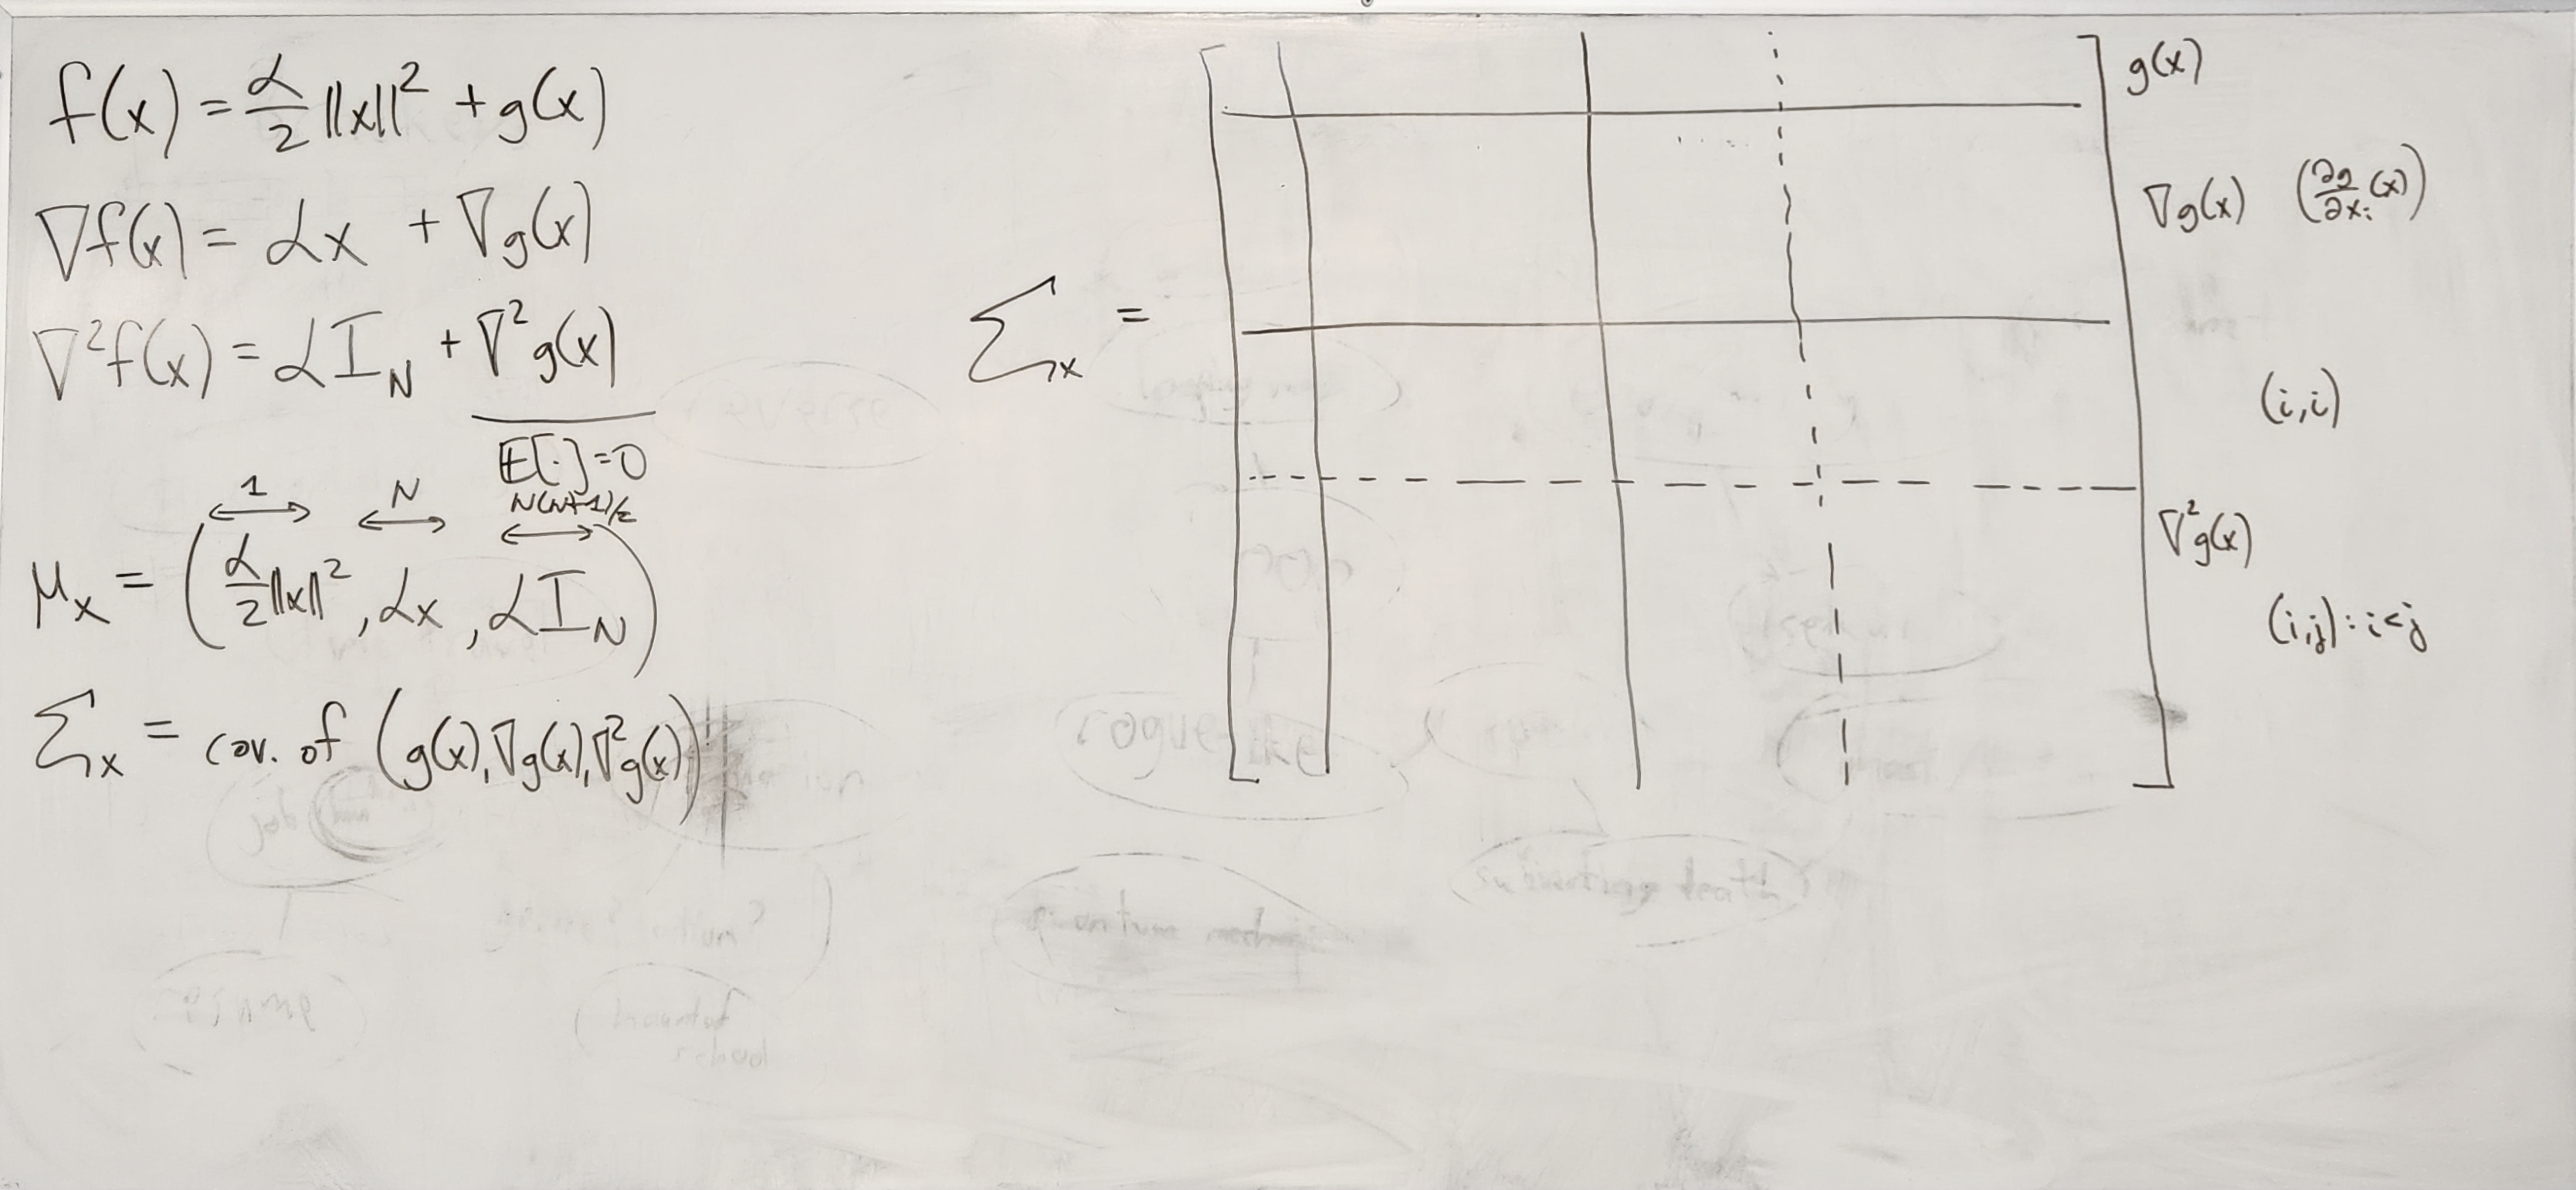
\includegraphics[width=\linewidth]{fig/empty_matrix.jpeg}
  \caption{A big covariance matrix.}
  \label{fig:empty matrix}
\end{figure}

\subsection{Covariance Computations}
Now,
taking an expectation is simply an integral.
In the case of ``nice'' functions,
we know from elementary calculus that we are able to exchange the order of the integral and differential.
Staring long enough yields the following identity.
\[
  \E\left[ \frac{\partial^a g}{\partial x_{i_1}\dots \partial x_{i_a}}(x) \frac{\partial^b g}{\partial y_{j_1}\dots \partial y_{j_b}}(y) \right]
  = \frac{\partial^{a+b} K}{\partial x_{i_1}\dots \partial x_{i_a} \partial y_{j_1}\dots \partial y_{j_b}} (x, y).
\]

\begin{figure}[h]
  \centering
  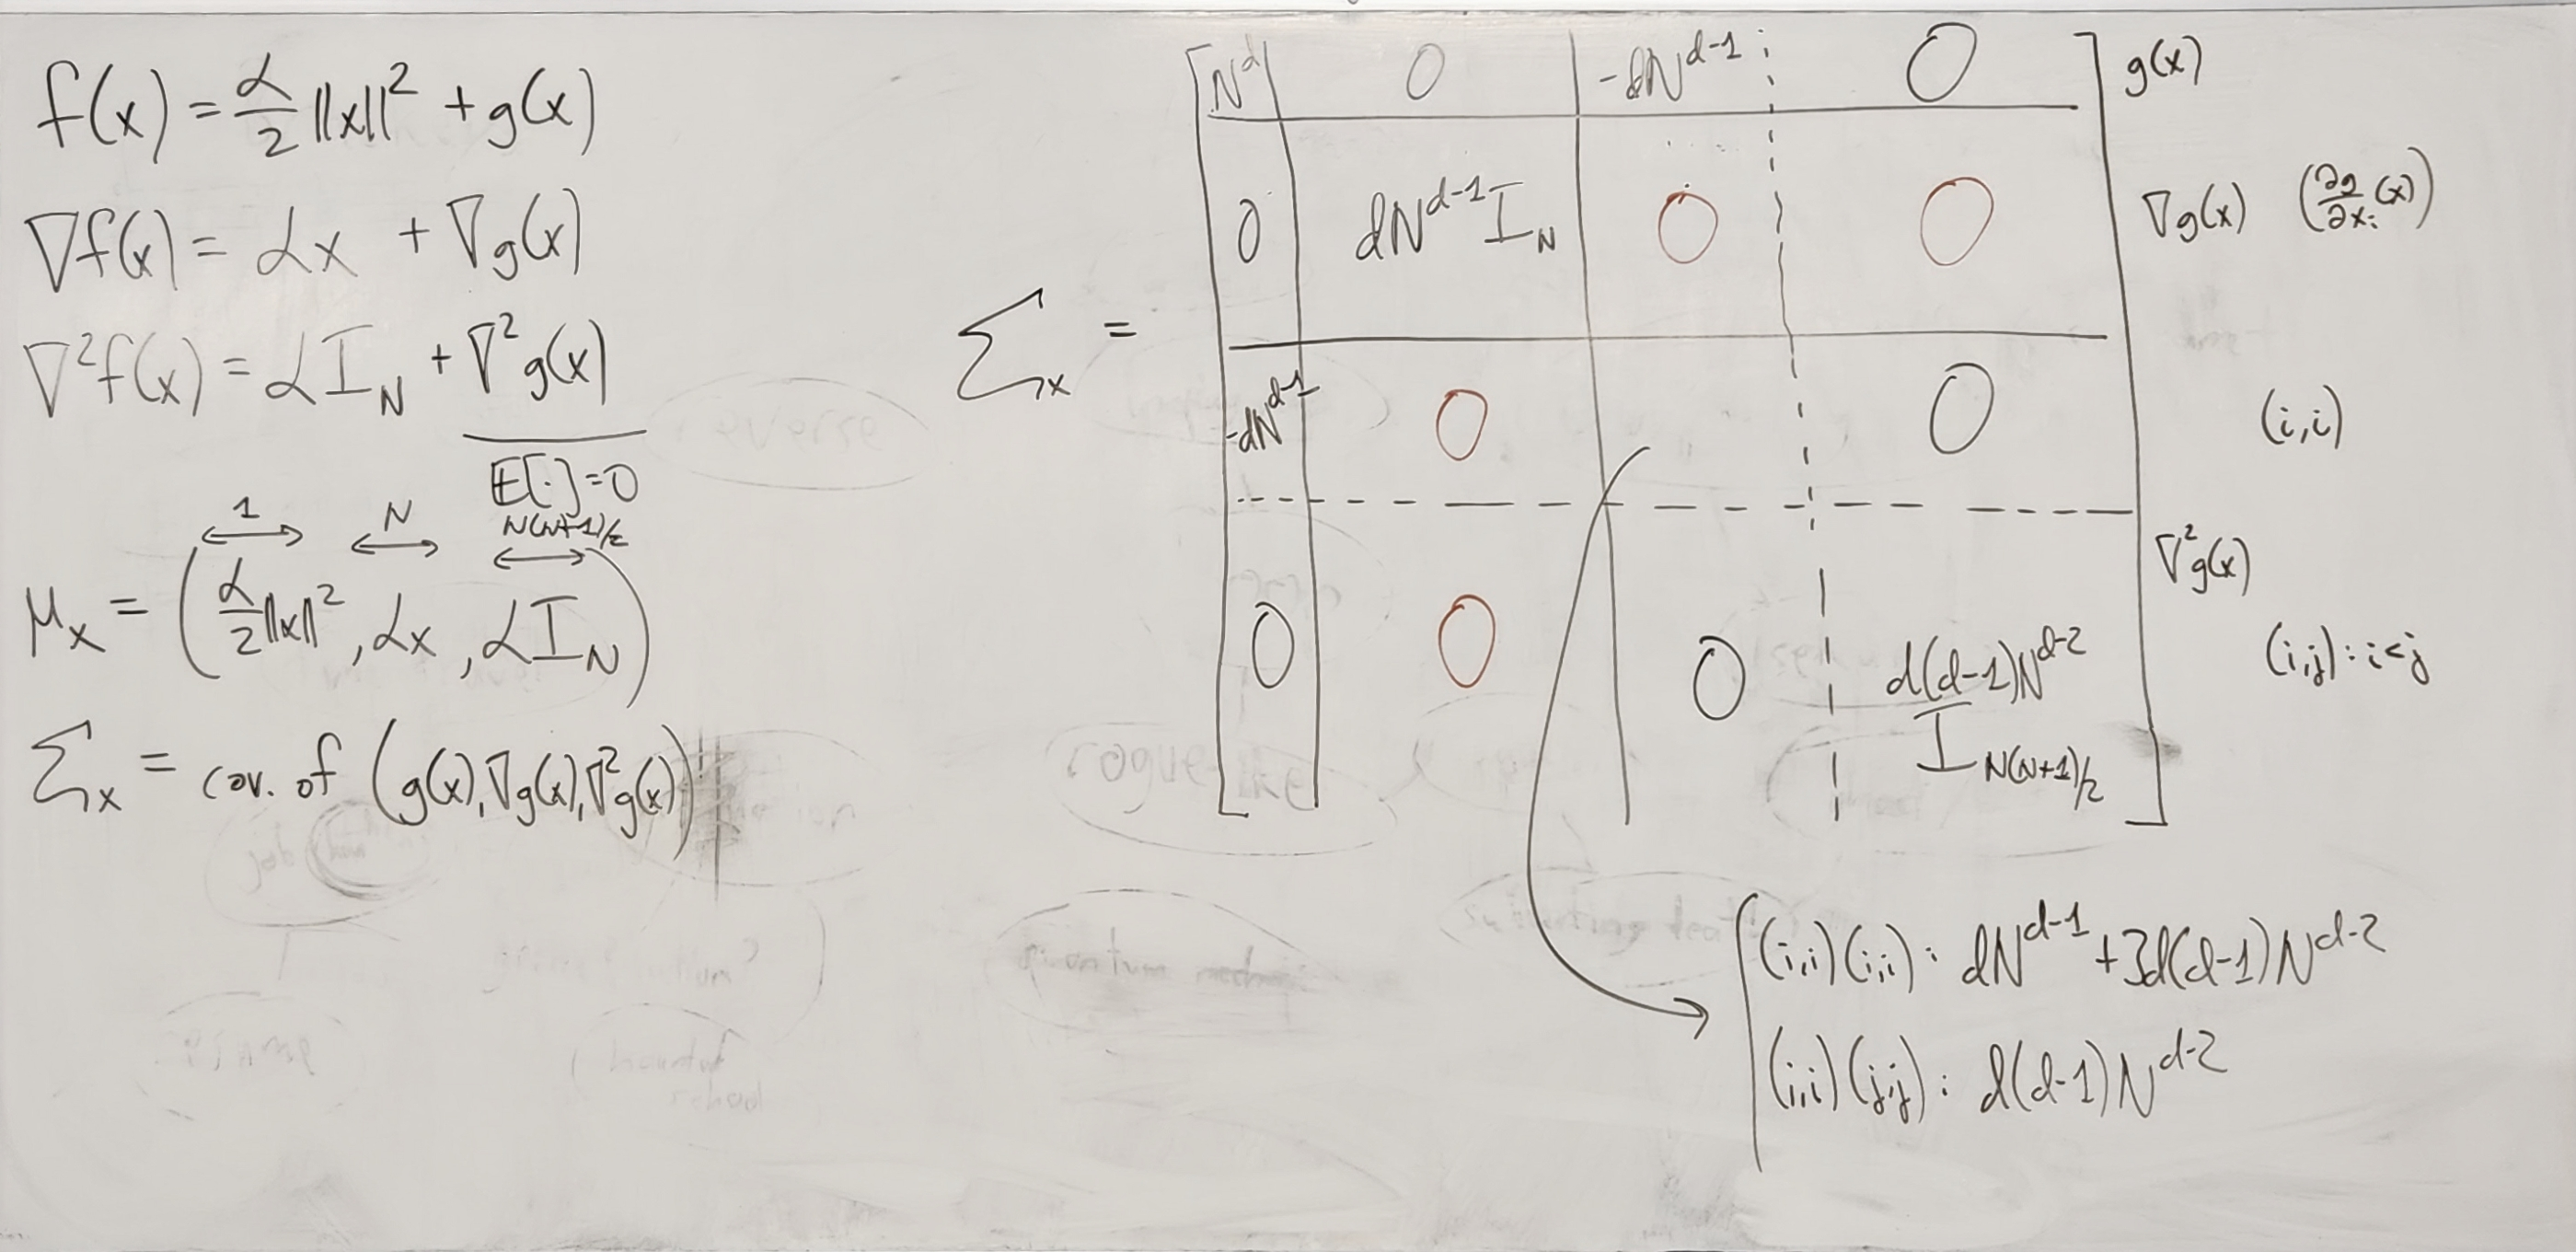
\includegraphics[width=\linewidth]{fig/filled_matrix.jpeg}
  \caption{A filled out covariance matrix.}
  \label{fig:filled matrix}
\end{figure}

\section{An Explicit Random Matrix Model}

\end{document}
